\documentclass[twoside]{book}

% Packages required by doxygen
\usepackage{fixltx2e}
\usepackage{calc}
\usepackage{doxygen}
\usepackage{graphicx}
\usepackage[utf8]{inputenc}
\usepackage{makeidx}
\usepackage{multicol}
\usepackage{multirow}
\PassOptionsToPackage{warn}{textcomp}
\usepackage{textcomp}
\usepackage[nointegrals]{wasysym}
\usepackage[table]{xcolor}

% Font selection
\usepackage[T1]{fontenc}
\usepackage{mathptmx}
\usepackage[scaled=.90]{helvet}
\usepackage{courier}
\usepackage{amssymb}
\usepackage{sectsty}
\renewcommand{\familydefault}{\sfdefault}
\allsectionsfont{%
  \fontseries{bc}\selectfont%
  \color{darkgray}%
}
\renewcommand{\DoxyLabelFont}{%
  \fontseries{bc}\selectfont%
  \color{darkgray}%
}
\newcommand{\+}{\discretionary{\mbox{\scriptsize$\hookleftarrow$}}{}{}}

% Page & text layout
\usepackage{geometry}
\geometry{%
  a4paper,%
  top=2.5cm,%
  bottom=2.5cm,%
  left=2.5cm,%
  right=2.5cm%
}
\tolerance=750
\hfuzz=15pt
\hbadness=750
\setlength{\emergencystretch}{15pt}
\setlength{\parindent}{0cm}
\setlength{\parskip}{0.2cm}
\makeatletter
\renewcommand{\paragraph}{%
  \@startsection{paragraph}{4}{0ex}{-1.0ex}{1.0ex}{%
    \normalfont\normalsize\bfseries\SS@parafont%
  }%
}
\renewcommand{\subparagraph}{%
  \@startsection{subparagraph}{5}{0ex}{-1.0ex}{1.0ex}{%
    \normalfont\normalsize\bfseries\SS@subparafont%
  }%
}
\makeatother

% Headers & footers
\usepackage{fancyhdr}
\pagestyle{fancyplain}
\fancyhead[LE]{\fancyplain{}{\bfseries\thepage}}
\fancyhead[CE]{\fancyplain{}{}}
\fancyhead[RE]{\fancyplain{}{\bfseries\leftmark}}
\fancyhead[LO]{\fancyplain{}{\bfseries\rightmark}}
\fancyhead[CO]{\fancyplain{}{}}
\fancyhead[RO]{\fancyplain{}{\bfseries\thepage}}
\fancyfoot[LE]{\fancyplain{}{}}
\fancyfoot[CE]{\fancyplain{}{}}
\fancyfoot[RE]{\fancyplain{}{\bfseries\scriptsize Generated on Sun Dec 18 2016 19\+:22\+:10 for Douglas the Dungeoneer by Doxygen }}
\fancyfoot[LO]{\fancyplain{}{\bfseries\scriptsize Generated on Sun Dec 18 2016 19\+:22\+:10 for Douglas the Dungeoneer by Doxygen }}
\fancyfoot[CO]{\fancyplain{}{}}
\fancyfoot[RO]{\fancyplain{}{}}
\renewcommand{\footrulewidth}{0.4pt}
\renewcommand{\chaptermark}[1]{%
  \markboth{#1}{}%
}
\renewcommand{\sectionmark}[1]{%
  \markright{\thesection\ #1}%
}

% Indices & bibliography
\usepackage{natbib}
\usepackage[titles]{tocloft}
\setcounter{tocdepth}{3}
\setcounter{secnumdepth}{5}
\makeindex

% Hyperlinks (required, but should be loaded last)
\usepackage{ifpdf}
\ifpdf
  \usepackage[pdftex,pagebackref=true]{hyperref}
\else
  \usepackage[ps2pdf,pagebackref=true]{hyperref}
\fi
\hypersetup{%
  colorlinks=true,%
  linkcolor=blue,%
  citecolor=blue,%
  unicode%
}

% Custom commands
\newcommand{\clearemptydoublepage}{%
  \newpage{\pagestyle{empty}\cleardoublepage}%
}


%===== C O N T E N T S =====

\begin{document}

% Titlepage & ToC
\hypersetup{pageanchor=false,
             bookmarks=true,
             bookmarksnumbered=true,
             pdfencoding=unicode
            }
\pagenumbering{roman}
\begin{titlepage}
\vspace*{7cm}
\begin{center}%
{\Large Douglas the Dungeoneer }\\
\vspace*{1cm}
{\large Generated by Doxygen 1.8.7}\\
\vspace*{0.5cm}
{\small Sun Dec 18 2016 19:22:10}\\
\end{center}
\end{titlepage}
\clearemptydoublepage
\tableofcontents
\clearemptydoublepage
\pagenumbering{arabic}
\hypersetup{pageanchor=true}

%--- Begin generated contents ---
\chapter{Hierarchical Index}
\section{Class Hierarchy}
This inheritance list is sorted roughly, but not completely, alphabetically\+:\begin{DoxyCompactList}
\item Drawable\begin{DoxyCompactList}
\item \contentsline{section}{Object}{\pageref{classObject}}{}
\begin{DoxyCompactList}
\item \contentsline{section}{Goal}{\pageref{classGoal}}{}
\item \contentsline{section}{Movable}{\pageref{classMovable}}{}
\begin{DoxyCompactList}
\item \contentsline{section}{Monster}{\pageref{classMonster}}{}
\item \contentsline{section}{Player}{\pageref{classPlayer}}{}
\end{DoxyCompactList}
\item \contentsline{section}{Treasure}{\pageref{classTreasure}}{}
\begin{DoxyCompactList}
\item \contentsline{section}{Equipment}{\pageref{classEquipment}}{}
\item \contentsline{section}{Gold}{\pageref{classGold}}{}
\item \contentsline{section}{Potion}{\pageref{classPotion}}{}
\end{DoxyCompactList}
\item \contentsline{section}{Wall}{\pageref{classWall}}{}
\end{DoxyCompactList}
\end{DoxyCompactList}
\item \contentsline{section}{Game}{\pageref{classGame}}{}
\item \contentsline{section}{Game\+\_\+\+State}{\pageref{classGame__State}}{}
\item \contentsline{section}{Level}{\pageref{classLevel}}{}
\end{DoxyCompactList}

\chapter{Class Index}
\section{Class List}
Here are the classes, structs, unions and interfaces with brief descriptions\+:\begin{DoxyCompactList}
\item\contentsline{section}{\hyperlink{classEquipment}{Equipment} }{\pageref{classEquipment}}{}
\item\contentsline{section}{\hyperlink{classGame}{Game} }{\pageref{classGame}}{}
\item\contentsline{section}{\hyperlink{classGame__State}{Game\+\_\+\+State} }{\pageref{classGame__State}}{}
\item\contentsline{section}{\hyperlink{classGoal}{Goal} }{\pageref{classGoal}}{}
\item\contentsline{section}{\hyperlink{classGold}{Gold} }{\pageref{classGold}}{}
\item\contentsline{section}{\hyperlink{classLevel}{Level} }{\pageref{classLevel}}{}
\item\contentsline{section}{\hyperlink{classMonster}{Monster} }{\pageref{classMonster}}{}
\item\contentsline{section}{\hyperlink{classMovable}{Movable} }{\pageref{classMovable}}{}
\item\contentsline{section}{\hyperlink{classObject}{Object} }{\pageref{classObject}}{}
\item\contentsline{section}{\hyperlink{classPlayer}{Player} }{\pageref{classPlayer}}{}
\item\contentsline{section}{\hyperlink{classPotion}{Potion} }{\pageref{classPotion}}{}
\item\contentsline{section}{\hyperlink{classTreasure}{Treasure} }{\pageref{classTreasure}}{}
\item\contentsline{section}{\hyperlink{classWall}{Wall} }{\pageref{classWall}}{}
\end{DoxyCompactList}

\chapter{Class Documentation}
\hypertarget{classEquipment}{\section{Equipment Class Reference}
\label{classEquipment}\index{Equipment@{Equipment}}
}


Inheritance diagram for Equipment\+:
\nopagebreak
\begin{figure}[H]
\begin{center}
\leavevmode
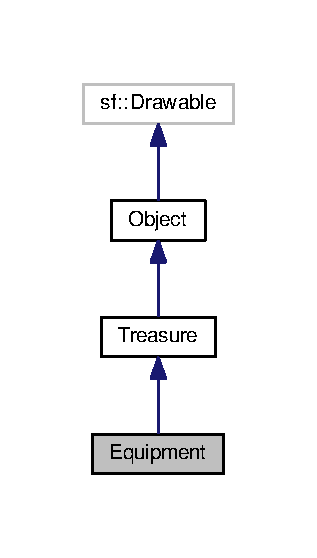
\includegraphics[width=152pt]{classEquipment__inherit__graph}
\end{center}
\end{figure}


Collaboration diagram for Equipment\+:
\nopagebreak
\begin{figure}[H]
\begin{center}
\leavevmode
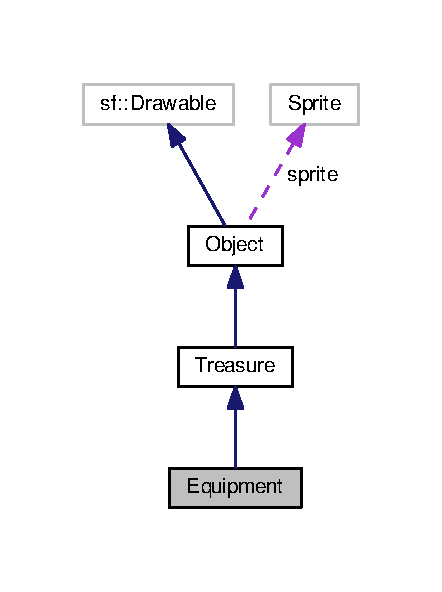
\includegraphics[width=212pt]{classEquipment__coll__graph}
\end{center}
\end{figure}
\subsection*{Public Member Functions}
\begin{DoxyCompactItemize}
\item 
\hyperlink{classEquipment_ae25b815e5d106e2053050da7818fd277}{Equipment} (int x\+\_\+val, int y\+\_\+val, int wid, int val, sf\+::\+Texture \&tex, sf\+::\+Int\+Rect rect)
\item 
virtual void \hyperlink{classEquipment_ae420383e1e845e886f60ffa6b6c82312}{collect} (\hyperlink{classPlayer}{Player} \&player) override
\end{DoxyCompactItemize}
\subsection*{Additional Inherited Members}


\subsection{Constructor \& Destructor Documentation}
\hypertarget{classEquipment_ae25b815e5d106e2053050da7818fd277}{\index{Equipment@{Equipment}!Equipment@{Equipment}}
\index{Equipment@{Equipment}!Equipment@{Equipment}}
\subsubsection[{Equipment}]{\setlength{\rightskip}{0pt plus 5cm}Equipment\+::\+Equipment (
\begin{DoxyParamCaption}
\item[{int}]{x\+\_\+val, }
\item[{int}]{y\+\_\+val, }
\item[{int}]{wid, }
\item[{int}]{val, }
\item[{sf\+::\+Texture \&}]{tex, }
\item[{sf\+::\+Int\+Rect}]{rect}
\end{DoxyParamCaption}
)}}\label{classEquipment_ae25b815e5d106e2053050da7818fd277}
\hyperlink{classEquipment}{Equipment} the player can collect to increase damage given and decrease damage taken 
\begin{DoxyParams}{Parameters}
{\em x\+\_\+val} & X coordinate of the equipment \\
\hline
{\em y\+\_\+val} & Y coordinate of the equipment \\
\hline
{\em wid} & Width of the equipment object \\
\hline
{\em val} & Value used to increase/decrease damage \\
\hline
{\em tex} & Tileset texture to create the sprite from \\
\hline
{\em rect} & Area of the tileset to create the sprite from \\
\hline
\end{DoxyParams}


\subsection{Member Function Documentation}
\hypertarget{classEquipment_ae420383e1e845e886f60ffa6b6c82312}{\index{Equipment@{Equipment}!collect@{collect}}
\index{collect@{collect}!Equipment@{Equipment}}
\subsubsection[{collect}]{\setlength{\rightskip}{0pt plus 5cm}void Equipment\+::collect (
\begin{DoxyParamCaption}
\item[{{\bf Player} \&}]{player}
\end{DoxyParamCaption}
)\hspace{0.3cm}{\ttfamily [override]}, {\ttfamily [virtual]}}}\label{classEquipment_ae420383e1e845e886f60ffa6b6c82312}
Calls on player's equip\+Treasure function with the equipment object's value variable as its parameter 
\begin{DoxyParams}{Parameters}
{\em player} & The player object that collects the equipment \\
\hline
\end{DoxyParams}


Implements \hyperlink{classTreasure_a55f46cc5e888315d78c423e6d0af102d}{Treasure}.



The documentation for this class was generated from the following files\+:\begin{DoxyCompactItemize}
\item 
equipment.\+h\item 
equipment.\+cpp\end{DoxyCompactItemize}

\hypertarget{classGame}{\section{Game Class Reference}
\label{classGame}\index{Game@{Game}}
}
\subsection*{Public Member Functions}
\begin{DoxyCompactItemize}
\item 
\hyperlink{classGame_a0a3902a3296afabb63deb10287205789}{Game} (int lvl, int play\+\_\+level, int play\+\_\+exp, int play\+\_\+score)
\item 
\hyperlink{classPlayer}{Player} \hyperlink{classGame_ab5d6f774a2722a4bffd9d1415871b8c7}{get\+Player} () const 
\item 
bool \hyperlink{classGame_abda2a003c77c17b87c44ab031060367a}{run} (Render\+Window \&window)
\end{DoxyCompactItemize}


\subsection{Constructor \& Destructor Documentation}
\hypertarget{classGame_a0a3902a3296afabb63deb10287205789}{\index{Game@{Game}!Game@{Game}}
\index{Game@{Game}!Game@{Game}}
\subsubsection[{Game}]{\setlength{\rightskip}{0pt plus 5cm}Game\+::\+Game (
\begin{DoxyParamCaption}
\item[{int}]{lvl, }
\item[{int}]{play\+\_\+level, }
\item[{int}]{play\+\_\+exp, }
\item[{int}]{play\+\_\+score}
\end{DoxyParamCaption}
)}}\label{classGame_a0a3902a3296afabb63deb10287205789}
Creates a \hyperlink{classGame}{Game} object able to play a \hyperlink{classLevel}{Level} 
\begin{DoxyParams}{Parameters}
{\em lvl} & The level number to play \\
\hline
{\em play\+\_\+level} & The starting level of the \hyperlink{classPlayer}{Player} \\
\hline
{\em play\+\_\+exp} & The starting experience of the \hyperlink{classPlayer}{Player} \\
\hline
{\em play\+\_\+score} & The starting score of the \hyperlink{classPlayer}{Player} \\
\hline
\end{DoxyParams}


\subsection{Member Function Documentation}
\hypertarget{classGame_ab5d6f774a2722a4bffd9d1415871b8c7}{\index{Game@{Game}!get\+Player@{get\+Player}}
\index{get\+Player@{get\+Player}!Game@{Game}}
\subsubsection[{get\+Player}]{\setlength{\rightskip}{0pt plus 5cm}{\bf Player} Game\+::get\+Player (
\begin{DoxyParamCaption}
{}
\end{DoxyParamCaption}
) const}}\label{classGame_ab5d6f774a2722a4bffd9d1415871b8c7}
\begin{DoxyReturn}{Returns}
The \hyperlink{classPlayer}{Player} object of the \hyperlink{classGame}{Game} 
\end{DoxyReturn}
\hypertarget{classGame_abda2a003c77c17b87c44ab031060367a}{\index{Game@{Game}!run@{run}}
\index{run@{run}!Game@{Game}}
\subsubsection[{run}]{\setlength{\rightskip}{0pt plus 5cm}bool Game\+::run (
\begin{DoxyParamCaption}
\item[{Render\+Window \&}]{window}
\end{DoxyParamCaption}
)}}\label{classGame_abda2a003c77c17b87c44ab031060367a}
Starts the game loop and sends events to the event handler 
\begin{DoxyParams}{Parameters}
{\em window} & The game window \\
\hline
\end{DoxyParams}
\begin{DoxyReturn}{Returns}
If the \hyperlink{classPlayer}{Player} is alive and the \hyperlink{classLevel}{Level} has been completed 
\end{DoxyReturn}


The documentation for this class was generated from the following files\+:\begin{DoxyCompactItemize}
\item 
game.\+h\item 
game.\+cpp\end{DoxyCompactItemize}

\hypertarget{classGame__State}{\section{Game\+\_\+\+State Class Reference}
\label{classGame__State}\index{Game\+\_\+\+State@{Game\+\_\+\+State}}
}
\subsection*{Public Member Functions}
\begin{DoxyCompactItemize}
\item 
\hyperlink{classGame__State_a8104ef051de61662ee5aef3f63c5d331}{Game\+\_\+\+State} ()
\item 
void \hyperlink{classGame__State_ab7ed16a10be9803ced8fee68e65085a1}{run} (sf\+::\+Render\+Window \&window)
\end{DoxyCompactItemize}


\subsection{Constructor \& Destructor Documentation}
\hypertarget{classGame__State_a8104ef051de61662ee5aef3f63c5d331}{\index{Game\+\_\+\+State@{Game\+\_\+\+State}!Game\+\_\+\+State@{Game\+\_\+\+State}}
\index{Game\+\_\+\+State@{Game\+\_\+\+State}!Game\+\_\+\+State@{Game\+\_\+\+State}}
\subsubsection[{Game\+\_\+\+State}]{\setlength{\rightskip}{0pt plus 5cm}Game\+\_\+\+State\+::\+Game\+\_\+\+State (
\begin{DoxyParamCaption}
{}
\end{DoxyParamCaption}
)}}\label{classGame__State_a8104ef051de61662ee5aef3f63c5d331}
Creates a \hyperlink{classGame__State}{Game\+\_\+\+State} that starts on level 1 and currently a total of 3 levels 

\subsection{Member Function Documentation}
\hypertarget{classGame__State_ab7ed16a10be9803ced8fee68e65085a1}{\index{Game\+\_\+\+State@{Game\+\_\+\+State}!run@{run}}
\index{run@{run}!Game\+\_\+\+State@{Game\+\_\+\+State}}
\subsubsection[{run}]{\setlength{\rightskip}{0pt plus 5cm}void Game\+\_\+\+State\+::run (
\begin{DoxyParamCaption}
\item[{sf\+::\+Render\+Window \&}]{window}
\end{DoxyParamCaption}
)}}\label{classGame__State_ab7ed16a10be9803ced8fee68e65085a1}
Starts the game loop, creating \hyperlink{classGame}{Game} objects until the player dies or the player has completed all available levels 
\begin{DoxyParams}{Parameters}
{\em window} & The window where the game is run \\
\hline
\end{DoxyParams}
If \hyperlink{classGame_abda2a003c77c17b87c44ab031060367a}{Game\+::run} returns false it means that the player has died or if the user has tried to close the window, which tells \hyperlink{classGame__State}{Game\+\_\+\+State} that the next level shouldn't be loaded

If the level is completed \hyperlink{classGame__State}{Game\+\_\+\+State} saves the player stats and loads them into the next level

The documentation for this class was generated from the following files\+:\begin{DoxyCompactItemize}
\item 
game\+\_\+state.\+h\item 
game\+\_\+state.\+cpp\end{DoxyCompactItemize}

\hypertarget{classGoal}{\section{Goal Class Reference}
\label{classGoal}\index{Goal@{Goal}}
}


Inheritance diagram for Goal\+:
\nopagebreak
\begin{figure}[H]
\begin{center}
\leavevmode
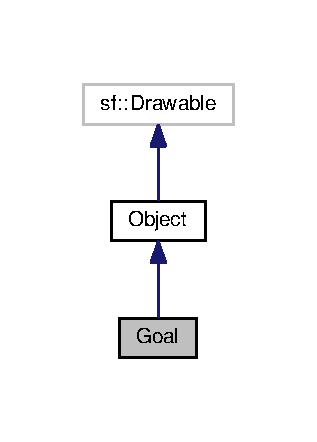
\includegraphics[width=152pt]{classGoal__inherit__graph}
\end{center}
\end{figure}


Collaboration diagram for Goal\+:
\nopagebreak
\begin{figure}[H]
\begin{center}
\leavevmode
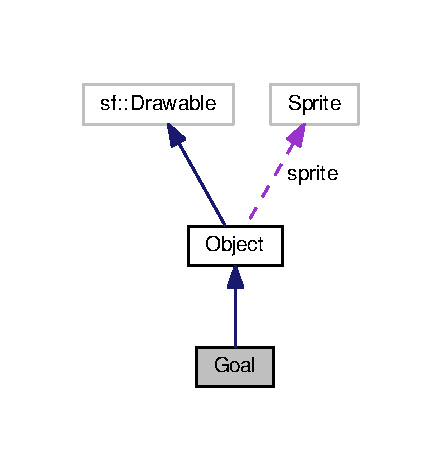
\includegraphics[width=212pt]{classGoal__coll__graph}
\end{center}
\end{figure}
\subsection*{Public Member Functions}
\begin{DoxyCompactItemize}
\item 
\hyperlink{classGoal_a579c482283005118e153af04d12d6326}{Goal} (int x\+\_\+val, int y\+\_\+val, int wid, sf\+::\+Texture \&tex, sf\+::\+Int\+Rect rect)
\item 
virtual bool \hyperlink{classGoal_ad23408eab330967a7fe0d13e580c667a}{active} () const override
\item 
void \hyperlink{classGoal_a4126af8f725af061df89124c1d9d2dfb}{end\+Game} ()
\item 
void \hyperlink{classGoal_adee29e993c9b988bd0cc15a12c86452d}{change\+Sprite} ()
\end{DoxyCompactItemize}
\subsection*{Additional Inherited Members}


\subsection{Constructor \& Destructor Documentation}
\hypertarget{classGoal_a579c482283005118e153af04d12d6326}{\index{Goal@{Goal}!Goal@{Goal}}
\index{Goal@{Goal}!Goal@{Goal}}
\subsubsection[{Goal}]{\setlength{\rightskip}{0pt plus 5cm}Goal\+::\+Goal (
\begin{DoxyParamCaption}
\item[{int}]{x\+\_\+val, }
\item[{int}]{y\+\_\+val, }
\item[{int}]{wid, }
\item[{sf\+::\+Texture \&}]{tex, }
\item[{sf\+::\+Int\+Rect}]{rect}
\end{DoxyParamCaption}
)}}\label{classGoal_a579c482283005118e153af04d12d6326}
Creates a goal object that knows if the 
\begin{DoxyParams}{Parameters}
{\em x\+\_\+val} & \\
\hline
{\em y\+\_\+val} & \\
\hline
{\em wid} & \\
\hline
{\em tex} & \\
\hline
{\em rect} & \\
\hline
\end{DoxyParams}


\subsection{Member Function Documentation}
\hypertarget{classGoal_ad23408eab330967a7fe0d13e580c667a}{\index{Goal@{Goal}!active@{active}}
\index{active@{active}!Goal@{Goal}}
\subsubsection[{active}]{\setlength{\rightskip}{0pt plus 5cm}bool Goal\+::active (
\begin{DoxyParamCaption}
{}
\end{DoxyParamCaption}
) const\hspace{0.3cm}{\ttfamily [override]}, {\ttfamily [virtual]}}}\label{classGoal_ad23408eab330967a7fe0d13e580c667a}
Checks if the level has been completed, either by the player dying or the player completing the level \begin{DoxyReturn}{Returns}
The value of finished 
\end{DoxyReturn}


Implements \hyperlink{classObject}{Object}.

\hypertarget{classGoal_adee29e993c9b988bd0cc15a12c86452d}{\index{Goal@{Goal}!change\+Sprite@{change\+Sprite}}
\index{change\+Sprite@{change\+Sprite}!Goal@{Goal}}
\subsubsection[{change\+Sprite}]{\setlength{\rightskip}{0pt plus 5cm}void Goal\+::change\+Sprite (
\begin{DoxyParamCaption}
{}
\end{DoxyParamCaption}
)}}\label{classGoal_adee29e993c9b988bd0cc15a12c86452d}
Changes the sprite to the open door sprite when the level is cleared of monsters and treasures \hypertarget{classGoal_a4126af8f725af061df89124c1d9d2dfb}{\index{Goal@{Goal}!end\+Game@{end\+Game}}
\index{end\+Game@{end\+Game}!Goal@{Goal}}
\subsubsection[{end\+Game}]{\setlength{\rightskip}{0pt plus 5cm}void Goal\+::end\+Game (
\begin{DoxyParamCaption}
{}
\end{DoxyParamCaption}
)}}\label{classGoal_a4126af8f725af061df89124c1d9d2dfb}
Sets the finished variable to true 

The documentation for this class was generated from the following files\+:\begin{DoxyCompactItemize}
\item 
goal.\+h\item 
goal.\+cpp\end{DoxyCompactItemize}

\hypertarget{classGold}{\section{Gold Class Reference}
\label{classGold}\index{Gold@{Gold}}
}


Inheritance diagram for Gold\+:
\nopagebreak
\begin{figure}[H]
\begin{center}
\leavevmode
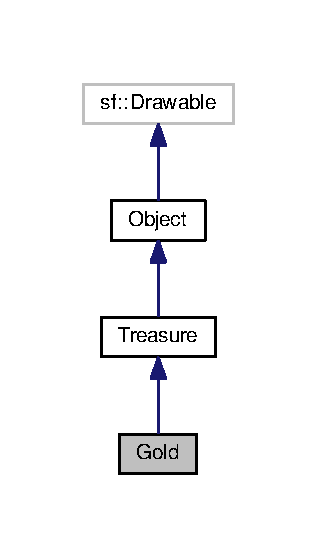
\includegraphics[width=152pt]{classGold__inherit__graph}
\end{center}
\end{figure}


Collaboration diagram for Gold\+:
\nopagebreak
\begin{figure}[H]
\begin{center}
\leavevmode
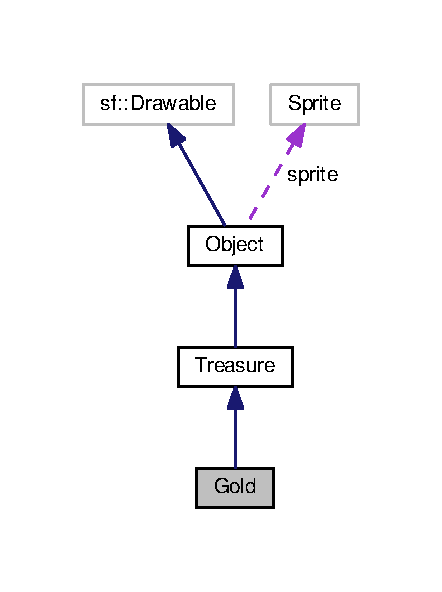
\includegraphics[width=212pt]{classGold__coll__graph}
\end{center}
\end{figure}
\subsection*{Public Member Functions}
\begin{DoxyCompactItemize}
\item 
\hyperlink{classGold_af4b58417b81cbc1632d5a15b8a4e125c}{Gold} (int x\+\_\+val, int y\+\_\+val, int wid, int val, sf\+::\+Texture \&tex, sf\+::\+Int\+Rect rect)
\item 
virtual void \hyperlink{classGold_a15403009146df6691835e27bbd5c0299}{collect} (\hyperlink{classPlayer}{Player} \&player) override
\end{DoxyCompactItemize}
\subsection*{Additional Inherited Members}


\subsection{Constructor \& Destructor Documentation}
\hypertarget{classGold_af4b58417b81cbc1632d5a15b8a4e125c}{\index{Gold@{Gold}!Gold@{Gold}}
\index{Gold@{Gold}!Gold@{Gold}}
\subsubsection[{Gold}]{\setlength{\rightskip}{0pt plus 5cm}Gold\+::\+Gold (
\begin{DoxyParamCaption}
\item[{int}]{x\+\_\+val, }
\item[{int}]{y\+\_\+val, }
\item[{int}]{wid, }
\item[{int}]{val, }
\item[{sf\+::\+Texture \&}]{tex, }
\item[{sf\+::\+Int\+Rect}]{rect}
\end{DoxyParamCaption}
)}}\label{classGold_af4b58417b81cbc1632d5a15b8a4e125c}
\hyperlink{classGold}{Gold} chests the player can collect to increase the score 
\begin{DoxyParams}{Parameters}
{\em x\+\_\+val} & X coordinate of the gold chest \\
\hline
{\em y\+\_\+val} & Y coordinate of the gold chest \\
\hline
{\em wid} & Width of the gold chest object \\
\hline
{\em val} & The value used to increase the score \\
\hline
{\em tex} & Tileset texture to create the sprite from \\
\hline
{\em rect} & Area of the tileset to create the sprite from \\
\hline
\end{DoxyParams}


\subsection{Member Function Documentation}
\hypertarget{classGold_a15403009146df6691835e27bbd5c0299}{\index{Gold@{Gold}!collect@{collect}}
\index{collect@{collect}!Gold@{Gold}}
\subsubsection[{collect}]{\setlength{\rightskip}{0pt plus 5cm}void Gold\+::collect (
\begin{DoxyParamCaption}
\item[{{\bf Player} \&}]{player}
\end{DoxyParamCaption}
)\hspace{0.3cm}{\ttfamily [override]}, {\ttfamily [virtual]}}}\label{classGold_a15403009146df6691835e27bbd5c0299}
Collects the treasure and increases player's score based on the \hyperlink{classGold}{Gold} object's value variable 
\begin{DoxyParams}{Parameters}
{\em player} & The \hyperlink{classPlayer}{Player} collecting the \hyperlink{classGold}{Gold} object \\
\hline
\end{DoxyParams}


Implements \hyperlink{classTreasure_a55f46cc5e888315d78c423e6d0af102d}{Treasure}.



The documentation for this class was generated from the following files\+:\begin{DoxyCompactItemize}
\item 
gold.\+h\item 
gold.\+cpp\end{DoxyCompactItemize}

\hypertarget{classLevel}{\section{Level Class Reference}
\label{classLevel}\index{Level@{Level}}
}
\subsection*{Public Member Functions}
\begin{DoxyCompactItemize}
\item 
\hyperlink{classLevel_a2646f8148d0a12d2e8f7eab310821fff}{Level} (int lvl)
\item 
Sprite \hyperlink{classLevel_a359be362457dd68d2ab3f1d97c2df15d}{get\+Bg} () const 
\item 
\hyperlink{classGoal}{Goal} \hyperlink{classLevel_acd10d8dbf30050291d9e61b369f107de}{get\+Goal} () const 
\item 
\hyperlink{classPlayer}{Player} \hyperlink{classLevel_a62dd39004dab7803646205824b171b35}{get\+Player} () const 
\item 
Sprite \hyperlink{classLevel_a7bf604cd9998a5810f2e8304b186b5cf}{get\+Status} () const 
\item 
vector$<$ \hyperlink{classWall}{Wall} $>$ \hyperlink{classLevel_a80193d2cc0acb2d5b35fd370c56c20b9}{get\+Walls} () const 
\item 
vector$<$ \hyperlink{classMonster}{Monster} $>$ \hyperlink{classLevel_a434cf5c4593a96e87ba0d48826f8f999}{get\+Monsters} () const 
\item 
vector$<$ \hyperlink{classTreasure}{Treasure} $\ast$ $>$ \hyperlink{classLevel_abab783b0e3b7b26b4a09e6fcbf0fb278}{get\+Treasures} () const 
\end{DoxyCompactItemize}


\subsection{Constructor \& Destructor Documentation}
\hypertarget{classLevel_a2646f8148d0a12d2e8f7eab310821fff}{\index{Level@{Level}!Level@{Level}}
\index{Level@{Level}!Level@{Level}}
\subsubsection[{Level}]{\setlength{\rightskip}{0pt plus 5cm}Level\+::\+Level (
\begin{DoxyParamCaption}
\item[{int}]{lvl}
\end{DoxyParamCaption}
)}}\label{classLevel_a2646f8148d0a12d2e8f7eab310821fff}
Loads the tilesets and then calls on read\+Level with the parameter l 
\begin{DoxyParams}{Parameters}
{\em l} & The number of the level to generate \\
\hline
\end{DoxyParams}
This tileset is made by the user Buch, \href{http://opengameart.org/users/buch,}{\tt http\+://opengameart.\+org/users/buch,} from opengameart.\+org and is available for download at\+: \href{http://opengameart.org/content/dungeon-tileset}{\tt http\+://opengameart.\+org/content/dungeon-\/tileset}

License\+: Public Domain \href{https://creativecommons.org/publicdomain/zero/1.0/}{\tt https\+://creativecommons.\+org/publicdomain/zero/1.\+0/}

This tileset is made by the user Buch, \href{http://opengameart.org/users/buch,}{\tt http\+://opengameart.\+org/users/buch,} from opengameart.\+org and is available for download at\+: \href{http://opengameart.org/content/rpg-items}{\tt http\+://opengameart.\+org/content/rpg-\/items}

License\+: Public Domain \href{https://creativecommons.org/publicdomain/zero/1.0/}{\tt https\+://creativecommons.\+org/publicdomain/zero/1.\+0/}

\subsection{Member Function Documentation}
\hypertarget{classLevel_a359be362457dd68d2ab3f1d97c2df15d}{\index{Level@{Level}!get\+Bg@{get\+Bg}}
\index{get\+Bg@{get\+Bg}!Level@{Level}}
\subsubsection[{get\+Bg}]{\setlength{\rightskip}{0pt plus 5cm}Sprite Level\+::get\+Bg (
\begin{DoxyParamCaption}
{}
\end{DoxyParamCaption}
) const}}\label{classLevel_a359be362457dd68d2ab3f1d97c2df15d}
\begin{DoxyReturn}{Returns}
The background sprite of the level 
\end{DoxyReturn}
\hypertarget{classLevel_acd10d8dbf30050291d9e61b369f107de}{\index{Level@{Level}!get\+Goal@{get\+Goal}}
\index{get\+Goal@{get\+Goal}!Level@{Level}}
\subsubsection[{get\+Goal}]{\setlength{\rightskip}{0pt plus 5cm}{\bf Goal} Level\+::get\+Goal (
\begin{DoxyParamCaption}
{}
\end{DoxyParamCaption}
) const}}\label{classLevel_acd10d8dbf30050291d9e61b369f107de}
\begin{DoxyReturn}{Returns}
The \hyperlink{classGoal}{Goal} object of the level 
\end{DoxyReturn}
\hypertarget{classLevel_a434cf5c4593a96e87ba0d48826f8f999}{\index{Level@{Level}!get\+Monsters@{get\+Monsters}}
\index{get\+Monsters@{get\+Monsters}!Level@{Level}}
\subsubsection[{get\+Monsters}]{\setlength{\rightskip}{0pt plus 5cm}vector$<$ {\bf Monster} $>$ Level\+::get\+Monsters (
\begin{DoxyParamCaption}
{}
\end{DoxyParamCaption}
) const}}\label{classLevel_a434cf5c4593a96e87ba0d48826f8f999}
\begin{DoxyReturn}{Returns}
The vector of all the monsters of the level 
\end{DoxyReturn}
\hypertarget{classLevel_a62dd39004dab7803646205824b171b35}{\index{Level@{Level}!get\+Player@{get\+Player}}
\index{get\+Player@{get\+Player}!Level@{Level}}
\subsubsection[{get\+Player}]{\setlength{\rightskip}{0pt plus 5cm}{\bf Player} Level\+::get\+Player (
\begin{DoxyParamCaption}
{}
\end{DoxyParamCaption}
) const}}\label{classLevel_a62dd39004dab7803646205824b171b35}
\begin{DoxyReturn}{Returns}
The \hyperlink{classPlayer}{Player} object of the level 
\end{DoxyReturn}
\hypertarget{classLevel_a7bf604cd9998a5810f2e8304b186b5cf}{\index{Level@{Level}!get\+Status@{get\+Status}}
\index{get\+Status@{get\+Status}!Level@{Level}}
\subsubsection[{get\+Status}]{\setlength{\rightskip}{0pt plus 5cm}Sprite Level\+::get\+Status (
\begin{DoxyParamCaption}
{}
\end{DoxyParamCaption}
) const}}\label{classLevel_a7bf604cd9998a5810f2e8304b186b5cf}
\begin{DoxyReturn}{Returns}
The status box sprite of the level 
\end{DoxyReturn}
\hypertarget{classLevel_abab783b0e3b7b26b4a09e6fcbf0fb278}{\index{Level@{Level}!get\+Treasures@{get\+Treasures}}
\index{get\+Treasures@{get\+Treasures}!Level@{Level}}
\subsubsection[{get\+Treasures}]{\setlength{\rightskip}{0pt plus 5cm}vector$<$ {\bf Treasure} $\ast$ $>$ Level\+::get\+Treasures (
\begin{DoxyParamCaption}
{}
\end{DoxyParamCaption}
) const}}\label{classLevel_abab783b0e3b7b26b4a09e6fcbf0fb278}
\begin{DoxyReturn}{Returns}
The vector of all of the treasures of the level 
\end{DoxyReturn}
\hypertarget{classLevel_a80193d2cc0acb2d5b35fd370c56c20b9}{\index{Level@{Level}!get\+Walls@{get\+Walls}}
\index{get\+Walls@{get\+Walls}!Level@{Level}}
\subsubsection[{get\+Walls}]{\setlength{\rightskip}{0pt plus 5cm}vector$<$ {\bf Wall} $>$ Level\+::get\+Walls (
\begin{DoxyParamCaption}
{}
\end{DoxyParamCaption}
) const}}\label{classLevel_a80193d2cc0acb2d5b35fd370c56c20b9}
\begin{DoxyReturn}{Returns}
The vector of all the walls of the level 
\end{DoxyReturn}


The documentation for this class was generated from the following files\+:\begin{DoxyCompactItemize}
\item 
level.\+h\item 
level.\+cpp\end{DoxyCompactItemize}

\hypertarget{classMonster}{\section{Monster Class Reference}
\label{classMonster}\index{Monster@{Monster}}
}


Inheritance diagram for Monster\+:
\nopagebreak
\begin{figure}[H]
\begin{center}
\leavevmode
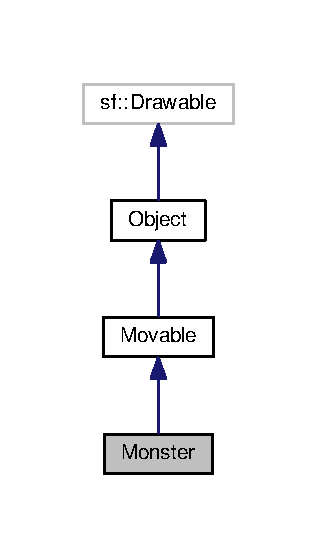
\includegraphics[width=152pt]{classMonster__inherit__graph}
\end{center}
\end{figure}


Collaboration diagram for Monster\+:
\nopagebreak
\begin{figure}[H]
\begin{center}
\leavevmode
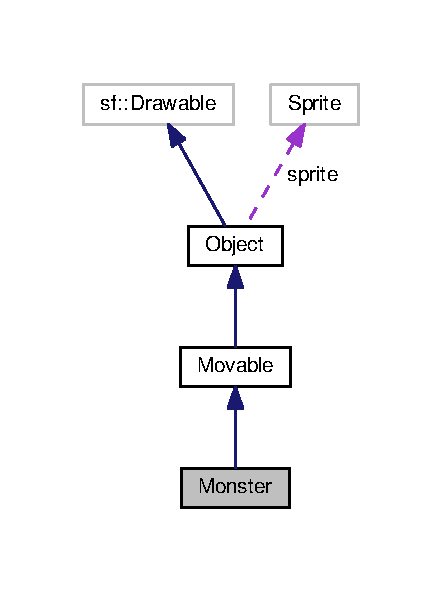
\includegraphics[width=212pt]{classMonster__coll__graph}
\end{center}
\end{figure}
\subsection*{Public Member Functions}
\begin{DoxyCompactItemize}
\item 
\hyperlink{classMonster_a975fd20f80f83dbc5dfc7bbcf5cb4cda}{Monster} (int x\+\_\+val, int y\+\_\+val, int wix, sf\+::\+Texture \&tex, sf\+::\+Int\+Rect \&rect, int max\+\_\+hp, int min\+\_\+att, int max\+\_\+att, std\+::vector$<$ std\+::pair$<$ int, int $>$$>$ route)
\item 
void \hyperlink{classMonster_a29d08fe330b6cad13e614693f1f3e16f}{move} ()
\item 
sf\+::\+Float\+Rect \hyperlink{classMonster_a1a595dfe12931dcd0ec4dbf41c8d22cc}{get\+Sight\+Box} () const 
\item 
virtual void \hyperlink{classMonster_a4185a3f93c9a4bdd9fa8caf95ffedab8}{attack} (\hyperlink{classMovable}{Movable} \&mov) override
\end{DoxyCompactItemize}
\subsection*{Additional Inherited Members}


\subsection{Constructor \& Destructor Documentation}
\hypertarget{classMonster_a975fd20f80f83dbc5dfc7bbcf5cb4cda}{\index{Monster@{Monster}!Monster@{Monster}}
\index{Monster@{Monster}!Monster@{Monster}}
\subsubsection[{Monster}]{\setlength{\rightskip}{0pt plus 5cm}Monster\+::\+Monster (
\begin{DoxyParamCaption}
\item[{int}]{x\+\_\+val, }
\item[{int}]{y\+\_\+val, }
\item[{int}]{wix, }
\item[{sf\+::\+Texture \&}]{tex, }
\item[{sf\+::\+Int\+Rect \&}]{rect, }
\item[{int}]{max\+\_\+hp, }
\item[{int}]{min\+\_\+att, }
\item[{int}]{max\+\_\+att, }
\item[{std\+::vector$<$ std\+::pair$<$ int, int $>$$>$}]{route}
\end{DoxyParamCaption}
)}}\label{classMonster_a975fd20f80f83dbc5dfc7bbcf5cb4cda}
A \hyperlink{classMonster}{Monster} object that patrols the level after a set cyclic route 
\begin{DoxyParams}{Parameters}
{\em x\+\_\+val} & X coordinate to spawn the player at \\
\hline
{\em y\+\_\+val} & Y coordinate to spawn the player at \\
\hline
{\em wid} & Width of the player object \\
\hline
{\em tex} & Texture used to create the player sprite \\
\hline
{\em rect} & Area of the texture to create the player sprite from \\
\hline
{\em max\+\_\+hp} & Max health points of the player object \\
\hline
{\em min\+\_\+att} & Minimum attack value of the player object \\
\hline
{\em max\+\_\+att} & Maximum attack value of the player object \\
\hline
{\em route} & The route the \hyperlink{classMonster}{Monster} will patrol \\
\hline
\end{DoxyParams}


\subsection{Member Function Documentation}
\hypertarget{classMonster_a4185a3f93c9a4bdd9fa8caf95ffedab8}{\index{Monster@{Monster}!attack@{attack}}
\index{attack@{attack}!Monster@{Monster}}
\subsubsection[{attack}]{\setlength{\rightskip}{0pt plus 5cm}void Monster\+::attack (
\begin{DoxyParamCaption}
\item[{{\bf Movable} \&}]{mov}
\end{DoxyParamCaption}
)\hspace{0.3cm}{\ttfamily [override]}, {\ttfamily [virtual]}}}\label{classMonster_a4185a3f93c9a4bdd9fa8caf95ffedab8}
Generates a value based on the \hyperlink{classMonster}{Monster}'s min\+\_\+attack and max\+\_\+attack variables. This value is doubled if a critical hit is generated, the value is then passed to mov's decrease\+H\+P function. 
\begin{DoxyParams}{Parameters}
{\em mov} & \hyperlink{classMovable}{Movable} attacked by the \hyperlink{classMonster}{Monster}. \\
\hline
\end{DoxyParams}


Implements \hyperlink{classMovable}{Movable}.

\hypertarget{classMonster_a1a595dfe12931dcd0ec4dbf41c8d22cc}{\index{Monster@{Monster}!get\+Sight\+Box@{get\+Sight\+Box}}
\index{get\+Sight\+Box@{get\+Sight\+Box}!Monster@{Monster}}
\subsubsection[{get\+Sight\+Box}]{\setlength{\rightskip}{0pt plus 5cm}sf\+::\+Float\+Rect Monster\+::get\+Sight\+Box (
\begin{DoxyParamCaption}
{}
\end{DoxyParamCaption}
) const}}\label{classMonster_a1a595dfe12931dcd0ec4dbf41c8d22cc}
Returns a Float\+Rect 3 times the \hyperlink{classMonster}{Monster}'s size surrounding it. Simple illustration, S is a part of the sight box while M is the \hyperlink{classMonster}{Monster} itself\+: S\+S\+S S\+M\+S S\+S\+S \begin{DoxyReturn}{Returns}
A Float\+Rect representing the \hyperlink{classMonster}{Monster} object's sight box 
\end{DoxyReturn}
\hypertarget{classMonster_a29d08fe330b6cad13e614693f1f3e16f}{\index{Monster@{Monster}!move@{move}}
\index{move@{move}!Monster@{Monster}}
\subsubsection[{move}]{\setlength{\rightskip}{0pt plus 5cm}void Monster\+::move (
\begin{DoxyParamCaption}
{}
\end{DoxyParamCaption}
)}}\label{classMonster_a29d08fe330b6cad13e614693f1f3e16f}
Moves the \hyperlink{classMonster}{Monster} to the next step of its patrol route unless the player intersects with the \hyperlink{classMonster}{Monster}'s sight box. The \hyperlink{classMonster}{Monster}'s sight box reaches one time the \hyperlink{classMonster}{Monster} object's width in all 8 directions. Step is the variable for which part of the patrol the monster is on, if the monster has completed its route step is set to 0 and the patrol resets

The documentation for this class was generated from the following files\+:\begin{DoxyCompactItemize}
\item 
monster.\+h\item 
monster.\+cc\end{DoxyCompactItemize}

\hypertarget{classMovable}{\section{Movable Class Reference}
\label{classMovable}\index{Movable@{Movable}}
}


Inheritance diagram for Movable\+:
\nopagebreak
\begin{figure}[H]
\begin{center}
\leavevmode
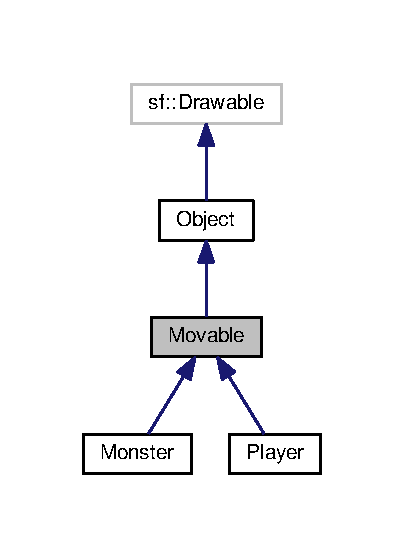
\includegraphics[width=194pt]{classMovable__inherit__graph}
\end{center}
\end{figure}


Collaboration diagram for Movable\+:
\nopagebreak
\begin{figure}[H]
\begin{center}
\leavevmode
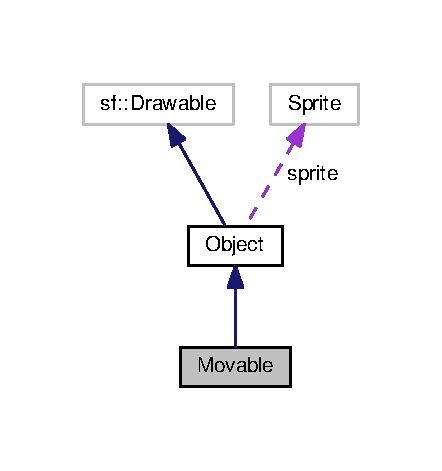
\includegraphics[width=212pt]{classMovable__coll__graph}
\end{center}
\end{figure}
\subsection*{Public Member Functions}
\begin{DoxyCompactItemize}
\item 
\hyperlink{classMovable_ab8074e1b870b06f5b7a2d93bc9f4a301}{Movable} (int x\+\_\+val, int y\+\_\+val, int wid, sf\+::\+Texture \&tex, sf\+::\+Int\+Rect \&rect, int max\+\_\+hp, int min\+\_\+att, int max\+\_\+att)
\item 
\hypertarget{classMovable_a6c90cd27651dcaae3673bf28bb9fa449}{virtual void {\bfseries attack} (\hyperlink{classMovable}{Movable} \&)=0}\label{classMovable_a6c90cd27651dcaae3673bf28bb9fa449}

\item 
void \hyperlink{classMovable_aa4f081848db7837daa7b6d6af25971bb}{decrease\+Hp} (int damage)
\item 
void \hyperlink{classMovable_ad247575b21471febb50f33cad3f7d5af}{heal} ()
\item 
virtual bool \hyperlink{classMovable_ad2c29da05cc65237d275e949cb4d6eb9}{active} () const override
\item 
void \hyperlink{classMovable_af86996f178b7acd13212d42bb3742c7c}{move} (int x\+\_\+move, int y\+\_\+move)
\end{DoxyCompactItemize}
\subsection*{Protected Attributes}
\begin{DoxyCompactItemize}
\item 
\hypertarget{classMovable_a0d351ec6b52976cfb30e811f9466c74c}{int {\bfseries equipment\+\_\+bonus} \{\}}\label{classMovable_a0d351ec6b52976cfb30e811f9466c74c}

\item 
\hypertarget{classMovable_a33933f3a87bdb382a3971946dec26573}{int {\bfseries max\+\_\+health} \{\}}\label{classMovable_a33933f3a87bdb382a3971946dec26573}

\item 
\hypertarget{classMovable_acebe27308e28f1a8ef1afc0975903277}{int {\bfseries current\+\_\+health} \{\}}\label{classMovable_acebe27308e28f1a8ef1afc0975903277}

\item 
\hypertarget{classMovable_ab89bbd5a67c47bc4a9c7f146df34fca5}{int {\bfseries min\+\_\+attack} \{\}}\label{classMovable_ab89bbd5a67c47bc4a9c7f146df34fca5}

\item 
\hypertarget{classMovable_a979c78acad9247d5d7ed7b7761c96c2f}{int {\bfseries max\+\_\+attack} \{\}}\label{classMovable_a979c78acad9247d5d7ed7b7761c96c2f}

\end{DoxyCompactItemize}


\subsection{Constructor \& Destructor Documentation}
\hypertarget{classMovable_ab8074e1b870b06f5b7a2d93bc9f4a301}{\index{Movable@{Movable}!Movable@{Movable}}
\index{Movable@{Movable}!Movable@{Movable}}
\subsubsection[{Movable}]{\setlength{\rightskip}{0pt plus 5cm}Movable\+::\+Movable (
\begin{DoxyParamCaption}
\item[{int}]{x\+\_\+val, }
\item[{int}]{y\+\_\+val, }
\item[{int}]{wid, }
\item[{sf\+::\+Texture \&}]{tex, }
\item[{sf\+::\+Int\+Rect \&}]{rect, }
\item[{int}]{max\+\_\+hp, }
\item[{int}]{min\+\_\+att, }
\item[{int}]{max\+\_\+att}
\end{DoxyParamCaption}
)}}\label{classMovable_ab8074e1b870b06f5b7a2d93bc9f4a301}
An abstract class for \hyperlink{classMovable}{Movable} objects 
\begin{DoxyParams}{Parameters}
{\em x\+\_\+val} & X coordinate to spawn the \hyperlink{classMovable}{Movable} at \\
\hline
{\em y\+\_\+val} & Y coordinate to spawn the \hyperlink{classMovable}{Movable} at \\
\hline
{\em wid} & Width of the \hyperlink{classMovable}{Movable} \\
\hline
{\em tex} & Texture used to create the \hyperlink{classMovable}{Movable} sprite \\
\hline
{\em rect} & Area of the texture to create the \hyperlink{classMovable}{Movable} sprite from \\
\hline
{\em max\+\_\+hp} & Max health points of the \hyperlink{classMovable}{Movable} object \\
\hline
{\em min\+\_\+att} & Minimum attack value of the \hyperlink{classMovable}{Movable} object \\
\hline
{\em max\+\_\+att} & Maximum attack value of the \hyperlink{classMovable}{Movable} object \\
\hline
\end{DoxyParams}


\subsection{Member Function Documentation}
\hypertarget{classMovable_ad2c29da05cc65237d275e949cb4d6eb9}{\index{Movable@{Movable}!active@{active}}
\index{active@{active}!Movable@{Movable}}
\subsubsection[{active}]{\setlength{\rightskip}{0pt plus 5cm}bool Movable\+::active (
\begin{DoxyParamCaption}
{}
\end{DoxyParamCaption}
) const\hspace{0.3cm}{\ttfamily [override]}, {\ttfamily [virtual]}}}\label{classMovable_ad2c29da05cc65237d275e949cb4d6eb9}
Checks if current\+\_\+health is greater than 0 \begin{DoxyReturn}{Returns}
current\+\_\+health $>$ 0 
\end{DoxyReturn}


Implements \hyperlink{classObject}{Object}.

\hypertarget{classMovable_aa4f081848db7837daa7b6d6af25971bb}{\index{Movable@{Movable}!decrease\+Hp@{decrease\+Hp}}
\index{decrease\+Hp@{decrease\+Hp}!Movable@{Movable}}
\subsubsection[{decrease\+Hp}]{\setlength{\rightskip}{0pt plus 5cm}void Movable\+::decrease\+Hp (
\begin{DoxyParamCaption}
\item[{int}]{damage}
\end{DoxyParamCaption}
)}}\label{classMovable_aa4f081848db7837daa7b6d6af25971bb}
Decreases current\+\_\+health by damage -\/ the value of the variable equipment\+\_\+bonus 
\begin{DoxyParams}{Parameters}
{\em damage} & The value to decrease current\+\_\+health by \\
\hline
\end{DoxyParams}
\hypertarget{classMovable_ad247575b21471febb50f33cad3f7d5af}{\index{Movable@{Movable}!heal@{heal}}
\index{heal@{heal}!Movable@{Movable}}
\subsubsection[{heal}]{\setlength{\rightskip}{0pt plus 5cm}void Movable\+::heal (
\begin{DoxyParamCaption}
{}
\end{DoxyParamCaption}
)}}\label{classMovable_ad247575b21471febb50f33cad3f7d5af}
Sets current\+\_\+health to the value of max\+\_\+health \hypertarget{classMovable_af86996f178b7acd13212d42bb3742c7c}{\index{Movable@{Movable}!move@{move}}
\index{move@{move}!Movable@{Movable}}
\subsubsection[{move}]{\setlength{\rightskip}{0pt plus 5cm}void Movable\+::move (
\begin{DoxyParamCaption}
\item[{int}]{x\+\_\+move, }
\item[{int}]{y\+\_\+move}
\end{DoxyParamCaption}
)}}\label{classMovable_af86996f178b7acd13212d42bb3742c7c}
Moves the \hyperlink{classMovable}{Movable} x\+\_\+move times its width on the X axis and y\+\_\+move times its width on the Y axis 
\begin{DoxyParams}{Parameters}
{\em x\+\_\+move} & The amount of steps to move on the X axis \\
\hline
{\em y\+\_\+move} & The amount of steps to move on the Y axis \\
\hline
\end{DoxyParams}


The documentation for this class was generated from the following files\+:\begin{DoxyCompactItemize}
\item 
movable.\+h\item 
movable.\+cc\end{DoxyCompactItemize}

\hypertarget{classObject}{\section{Object Class Reference}
\label{classObject}\index{Object@{Object}}
}


Inheritance diagram for Object\+:
\nopagebreak
\begin{figure}[H]
\begin{center}
\leavevmode
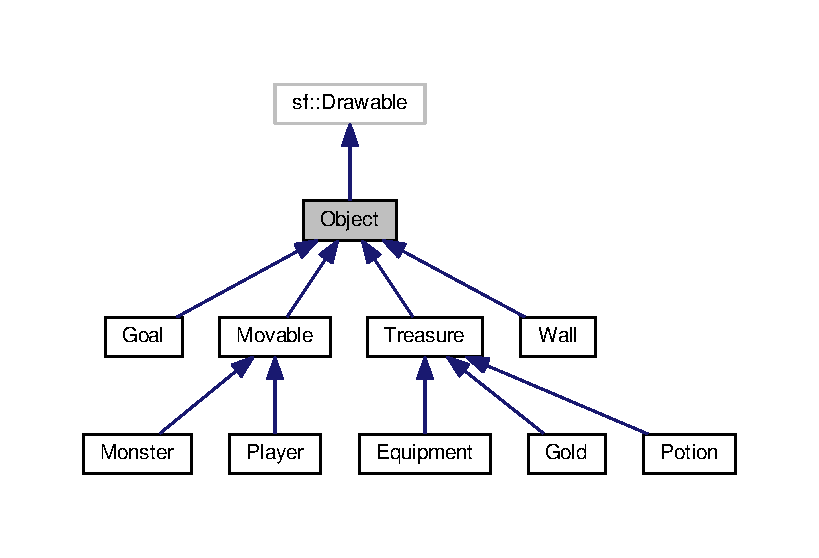
\includegraphics[width=350pt]{classObject__inherit__graph}
\end{center}
\end{figure}


Collaboration diagram for Object\+:
\nopagebreak
\begin{figure}[H]
\begin{center}
\leavevmode
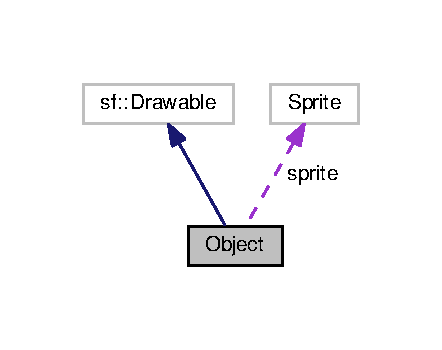
\includegraphics[width=212pt]{classObject__coll__graph}
\end{center}
\end{figure}
\subsection*{Public Member Functions}
\begin{DoxyCompactItemize}
\item 
\hyperlink{classObject_a5f8f752a3b0b7d68f15a5e2ff4d72f3b}{Object} (int x\+\_\+val, int y\+\_\+val, int wid, sf\+::\+Texture \&tex, sf\+::\+Int\+Rect rect)
\item 
\hypertarget{classObject_a097a320e7b93b92a27db87bb64bf5a63}{virtual bool {\bfseries active} () const =0}\label{classObject_a097a320e7b93b92a27db87bb64bf5a63}

\item 
sf\+::\+Sprite \hyperlink{classObject_a7541b5e9de4712cdb604035aaef66882}{get\+Sprite} () const 
\item 
virtual void \hyperlink{classObject_acfb343510263d8fb539979442e4e4e26}{draw} (sf\+::\+Render\+Target \&target, sf\+::\+Render\+States) const override
\end{DoxyCompactItemize}
\subsection*{Protected Attributes}
\begin{DoxyCompactItemize}
\item 
\hypertarget{classObject_a65be09abc56e93e0154c3a0e37f97579}{sf\+::\+Sprite {\bfseries sprite} \{\}}\label{classObject_a65be09abc56e93e0154c3a0e37f97579}

\item 
\hypertarget{classObject_aea8b4e1f4895ce5a0be5dbf42864669c}{int {\bfseries x} \{\}}\label{classObject_aea8b4e1f4895ce5a0be5dbf42864669c}

\item 
\hypertarget{classObject_a9ed372592e77352c832d721ad88b9aec}{int {\bfseries y} \{\}}\label{classObject_a9ed372592e77352c832d721ad88b9aec}

\item 
\hypertarget{classObject_a93596e8f620874b99326f8632365c8f5}{int {\bfseries width} \{\}}\label{classObject_a93596e8f620874b99326f8632365c8f5}

\end{DoxyCompactItemize}


\subsection{Constructor \& Destructor Documentation}
\hypertarget{classObject_a5f8f752a3b0b7d68f15a5e2ff4d72f3b}{\index{Object@{Object}!Object@{Object}}
\index{Object@{Object}!Object@{Object}}
\subsubsection[{Object}]{\setlength{\rightskip}{0pt plus 5cm}Object\+::\+Object (
\begin{DoxyParamCaption}
\item[{int}]{x\+\_\+val, }
\item[{int}]{y\+\_\+val, }
\item[{int}]{wid, }
\item[{sf\+::\+Texture \&}]{tex, }
\item[{sf\+::\+Int\+Rect}]{rect}
\end{DoxyParamCaption}
)}}\label{classObject_a5f8f752a3b0b7d68f15a5e2ff4d72f3b}
Creates an object with a position, width and sprite 
\begin{DoxyParams}{Parameters}
{\em x\+\_\+val} & X coordinate for the object \\
\hline
{\em y\+\_\+val} & Y coordinate for the object \\
\hline
{\em wid} & Width of the object \\
\hline
{\em tex} & Texture used to create the sprite \\
\hline
{\em rect} & The area of the texture to create the sprite from \\
\hline
\end{DoxyParams}


\subsection{Member Function Documentation}
\hypertarget{classObject_acfb343510263d8fb539979442e4e4e26}{\index{Object@{Object}!draw@{draw}}
\index{draw@{draw}!Object@{Object}}
\subsubsection[{draw}]{\setlength{\rightskip}{0pt plus 5cm}void Object\+::draw (
\begin{DoxyParamCaption}
\item[{sf\+::\+Render\+Target \&}]{target, }
\item[{sf\+::\+Render\+States}]{}
\end{DoxyParamCaption}
) const\hspace{0.3cm}{\ttfamily [override]}, {\ttfamily [virtual]}}}\label{classObject_acfb343510263d8fb539979442e4e4e26}
Draws the Ovject's sprite in the target, implementing this function has the effect that all objects of classes derived from \hyperlink{classObject}{Object} can be sent to a sf\+::\+Render\+Window's draw function directly and be drawn correctly in the window 
\begin{DoxyParams}{Parameters}
{\em target} & The Render\+Target to draw to \\
\hline
\end{DoxyParams}
\hypertarget{classObject_a7541b5e9de4712cdb604035aaef66882}{\index{Object@{Object}!get\+Sprite@{get\+Sprite}}
\index{get\+Sprite@{get\+Sprite}!Object@{Object}}
\subsubsection[{get\+Sprite}]{\setlength{\rightskip}{0pt plus 5cm}sf\+::\+Sprite Object\+::get\+Sprite (
\begin{DoxyParamCaption}
{}
\end{DoxyParamCaption}
) const}}\label{classObject_a7541b5e9de4712cdb604035aaef66882}
\begin{DoxyReturn}{Returns}
The sprite variable of the \hyperlink{classObject}{Object} 
\end{DoxyReturn}


The documentation for this class was generated from the following files\+:\begin{DoxyCompactItemize}
\item 
object.\+h\item 
object.\+cc\end{DoxyCompactItemize}

\hypertarget{classPlayer}{\section{Player Class Reference}
\label{classPlayer}\index{Player@{Player}}
}


Inheritance diagram for Player\+:
\nopagebreak
\begin{figure}[H]
\begin{center}
\leavevmode
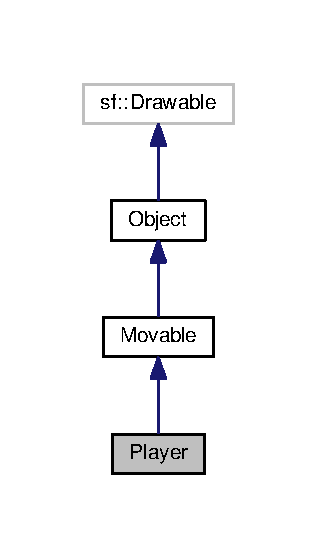
\includegraphics[width=152pt]{classPlayer__inherit__graph}
\end{center}
\end{figure}


Collaboration diagram for Player\+:
\nopagebreak
\begin{figure}[H]
\begin{center}
\leavevmode
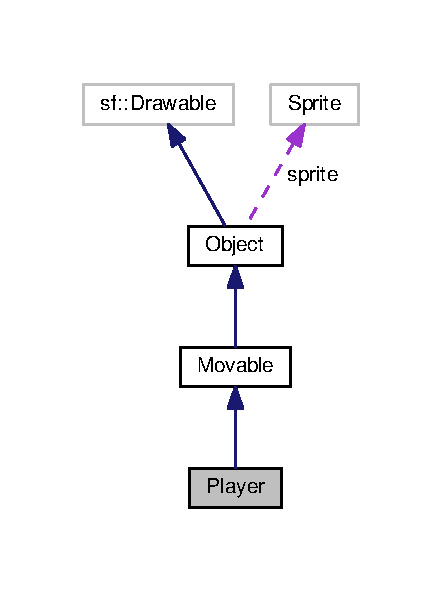
\includegraphics[width=212pt]{classPlayer__coll__graph}
\end{center}
\end{figure}
\subsection*{Public Member Functions}
\begin{DoxyCompactItemize}
\item 
\hyperlink{classPlayer_a3d096a675cddfcb4d2f74201bf7e3422}{Player} (int x\+\_\+val, int y\+\_\+val, int wid, sf\+::\+Texture \&tex, sf\+::\+Int\+Rect \&rect, int max\+\_\+hp, int min\+\_\+att, int max\+\_\+att)
\item 
virtual void \hyperlink{classPlayer_a8135c6f5b7c11fa3aa1c801d0219356a}{attack} (\hyperlink{classMovable}{Movable} \&mov) override
\item 
void \hyperlink{classPlayer_ab68186aa09a4b86263ec6b238b7d75c4}{increase\+Score} (int sco)
\item 
void \hyperlink{classPlayer_a5de85f52562c1630b8eba16f8384cc5a}{increase\+Experience} (int exp)
\item 
void \hyperlink{classPlayer_a4ccbbd0bf0c7a811c7765ea1b8d83240}{equip\+Treasure} (int val)
\item 
int \hyperlink{classPlayer_ac10eb9fb0387f565134958d129585ac6}{get\+Score} () const 
\item 
int \hyperlink{classPlayer_a54051098b038fa4d040b5d316fb3587a}{get\+Experience\+Points} () const 
\item 
int \hyperlink{classPlayer_a3042adb49808b2629137f4d85b6b5fd3}{get\+Health} () const 
\item 
int \hyperlink{classPlayer_ac963622d4c47bd62f142fa1bc34d39f9}{get\+Max\+Health} () const 
\item 
int \hyperlink{classPlayer_a9a41d6af9786e15212a821072b0395b2}{get\+Level} () const 
\item 
void \hyperlink{classPlayer_a16abe3e019dec51bdcfb3175c6721ce5}{set\+Level} (int val)
\item 
void \hyperlink{classPlayer_a71f00c57a2c8490d1f2716e9cf8ed172}{set\+Experience} (int exp)
\item 
void \hyperlink{classPlayer_adac972269da71038ba2442d9323b5c16}{set\+Score} (int sco)
\end{DoxyCompactItemize}
\subsection*{Additional Inherited Members}


\subsection{Constructor \& Destructor Documentation}
\hypertarget{classPlayer_a3d096a675cddfcb4d2f74201bf7e3422}{\index{Player@{Player}!Player@{Player}}
\index{Player@{Player}!Player@{Player}}
\subsubsection[{Player}]{\setlength{\rightskip}{0pt plus 5cm}Player\+::\+Player (
\begin{DoxyParamCaption}
\item[{int}]{x\+\_\+val, }
\item[{int}]{y\+\_\+val, }
\item[{int}]{wid, }
\item[{sf\+::\+Texture \&}]{tex, }
\item[{sf\+::\+Int\+Rect \&}]{rect, }
\item[{int}]{max\+\_\+hp, }
\item[{int}]{min\+\_\+att, }
\item[{int}]{max\+\_\+att}
\end{DoxyParamCaption}
)}}\label{classPlayer_a3d096a675cddfcb4d2f74201bf7e3422}
The player object that the player can control 
\begin{DoxyParams}{Parameters}
{\em x\+\_\+val} & X coordinate to spawn the player at \\
\hline
{\em y\+\_\+val} & Y coordinate to spawn the player at \\
\hline
{\em wid} & Width of the player object \\
\hline
{\em tex} & Texture used to create the player sprite \\
\hline
{\em rect} & Area of the texture to create the player sprite from \\
\hline
{\em max\+\_\+hp} & Max health points of the player object \\
\hline
{\em min\+\_\+att} & Minimum attack value of the player object \\
\hline
{\em max\+\_\+att} & Maximum attack value of the player object \\
\hline
\end{DoxyParams}


\subsection{Member Function Documentation}
\hypertarget{classPlayer_a8135c6f5b7c11fa3aa1c801d0219356a}{\index{Player@{Player}!attack@{attack}}
\index{attack@{attack}!Player@{Player}}
\subsubsection[{attack}]{\setlength{\rightskip}{0pt plus 5cm}void Player\+::attack (
\begin{DoxyParamCaption}
\item[{{\bf Movable} \&}]{mov}
\end{DoxyParamCaption}
)\hspace{0.3cm}{\ttfamily [override]}, {\ttfamily [virtual]}}}\label{classPlayer_a8135c6f5b7c11fa3aa1c801d0219356a}
Generates a value based on the player's min\+\_\+attack, max\+\_\+attack and level variables. This value is doubled if a critical hit is generated, the value is then passed to mov's decrease\+H\+P function. 
\begin{DoxyParams}{Parameters}
{\em mov} & \hyperlink{classMovable}{Movable} attacked by the player. \\
\hline
\end{DoxyParams}


Implements \hyperlink{classMovable}{Movable}.

\hypertarget{classPlayer_a4ccbbd0bf0c7a811c7765ea1b8d83240}{\index{Player@{Player}!equip\+Treasure@{equip\+Treasure}}
\index{equip\+Treasure@{equip\+Treasure}!Player@{Player}}
\subsubsection[{equip\+Treasure}]{\setlength{\rightskip}{0pt plus 5cm}void Player\+::equip\+Treasure (
\begin{DoxyParamCaption}
\item[{int}]{val}
\end{DoxyParamCaption}
)}}\label{classPlayer_a4ccbbd0bf0c7a811c7765ea1b8d83240}
Increases the equipment\+\_\+bonus variable with the value of val 
\begin{DoxyParams}{Parameters}
{\em val} & The value used to increase the equipment\+\_\+bonus variable \\
\hline
\end{DoxyParams}
\hypertarget{classPlayer_a54051098b038fa4d040b5d316fb3587a}{\index{Player@{Player}!get\+Experience\+Points@{get\+Experience\+Points}}
\index{get\+Experience\+Points@{get\+Experience\+Points}!Player@{Player}}
\subsubsection[{get\+Experience\+Points}]{\setlength{\rightskip}{0pt plus 5cm}int Player\+::get\+Experience\+Points (
\begin{DoxyParamCaption}
{}
\end{DoxyParamCaption}
) const}}\label{classPlayer_a54051098b038fa4d040b5d316fb3587a}
\begin{DoxyReturn}{Returns}
The \hyperlink{classPlayer}{Player} experience\+\_\+points variable 
\end{DoxyReturn}
\hypertarget{classPlayer_a3042adb49808b2629137f4d85b6b5fd3}{\index{Player@{Player}!get\+Health@{get\+Health}}
\index{get\+Health@{get\+Health}!Player@{Player}}
\subsubsection[{get\+Health}]{\setlength{\rightskip}{0pt plus 5cm}int Player\+::get\+Health (
\begin{DoxyParamCaption}
{}
\end{DoxyParamCaption}
) const}}\label{classPlayer_a3042adb49808b2629137f4d85b6b5fd3}
\begin{DoxyReturn}{Returns}
The \hyperlink{classPlayer}{Player} current\+\_\+health variable 
\end{DoxyReturn}
\hypertarget{classPlayer_a9a41d6af9786e15212a821072b0395b2}{\index{Player@{Player}!get\+Level@{get\+Level}}
\index{get\+Level@{get\+Level}!Player@{Player}}
\subsubsection[{get\+Level}]{\setlength{\rightskip}{0pt plus 5cm}int Player\+::get\+Level (
\begin{DoxyParamCaption}
{}
\end{DoxyParamCaption}
) const}}\label{classPlayer_a9a41d6af9786e15212a821072b0395b2}
\begin{DoxyReturn}{Returns}
The \hyperlink{classPlayer}{Player} level variable 
\end{DoxyReturn}
\hypertarget{classPlayer_ac963622d4c47bd62f142fa1bc34d39f9}{\index{Player@{Player}!get\+Max\+Health@{get\+Max\+Health}}
\index{get\+Max\+Health@{get\+Max\+Health}!Player@{Player}}
\subsubsection[{get\+Max\+Health}]{\setlength{\rightskip}{0pt plus 5cm}int Player\+::get\+Max\+Health (
\begin{DoxyParamCaption}
{}
\end{DoxyParamCaption}
) const}}\label{classPlayer_ac963622d4c47bd62f142fa1bc34d39f9}
\begin{DoxyReturn}{Returns}
The \hyperlink{classPlayer}{Player} max\+\_\+health variable 
\end{DoxyReturn}
\hypertarget{classPlayer_ac10eb9fb0387f565134958d129585ac6}{\index{Player@{Player}!get\+Score@{get\+Score}}
\index{get\+Score@{get\+Score}!Player@{Player}}
\subsubsection[{get\+Score}]{\setlength{\rightskip}{0pt plus 5cm}int Player\+::get\+Score (
\begin{DoxyParamCaption}
{}
\end{DoxyParamCaption}
) const}}\label{classPlayer_ac10eb9fb0387f565134958d129585ac6}
\begin{DoxyReturn}{Returns}
The \hyperlink{classPlayer}{Player} score variable 
\end{DoxyReturn}
\hypertarget{classPlayer_a5de85f52562c1630b8eba16f8384cc5a}{\index{Player@{Player}!increase\+Experience@{increase\+Experience}}
\index{increase\+Experience@{increase\+Experience}!Player@{Player}}
\subsubsection[{increase\+Experience}]{\setlength{\rightskip}{0pt plus 5cm}void Player\+::increase\+Experience (
\begin{DoxyParamCaption}
\item[{int}]{exp}
\end{DoxyParamCaption}
)}}\label{classPlayer_a5de85f52562c1630b8eba16f8384cc5a}
Increases the experience\+\_\+points variable with the value of exp 
\begin{DoxyParams}{Parameters}
{\em exp} & The value used to increase the experience\+\_\+points variable \\
\hline
\end{DoxyParams}
\hypertarget{classPlayer_ab68186aa09a4b86263ec6b238b7d75c4}{\index{Player@{Player}!increase\+Score@{increase\+Score}}
\index{increase\+Score@{increase\+Score}!Player@{Player}}
\subsubsection[{increase\+Score}]{\setlength{\rightskip}{0pt plus 5cm}void Player\+::increase\+Score (
\begin{DoxyParamCaption}
\item[{int}]{sco}
\end{DoxyParamCaption}
)}}\label{classPlayer_ab68186aa09a4b86263ec6b238b7d75c4}
Increases the score variable with the value of sco 
\begin{DoxyParams}{Parameters}
{\em sco} & The value used to increase the score variable \\
\hline
\end{DoxyParams}
\hypertarget{classPlayer_a71f00c57a2c8490d1f2716e9cf8ed172}{\index{Player@{Player}!set\+Experience@{set\+Experience}}
\index{set\+Experience@{set\+Experience}!Player@{Player}}
\subsubsection[{set\+Experience}]{\setlength{\rightskip}{0pt plus 5cm}void Player\+::set\+Experience (
\begin{DoxyParamCaption}
\item[{int}]{exp}
\end{DoxyParamCaption}
)}}\label{classPlayer_a71f00c57a2c8490d1f2716e9cf8ed172}
Sets the experience\+\_\+points variable to exp 
\begin{DoxyParams}{Parameters}
{\em exp} & Value used to set the value of experience\+\_\+points \\
\hline
\end{DoxyParams}
\hypertarget{classPlayer_a16abe3e019dec51bdcfb3175c6721ce5}{\index{Player@{Player}!set\+Level@{set\+Level}}
\index{set\+Level@{set\+Level}!Player@{Player}}
\subsubsection[{set\+Level}]{\setlength{\rightskip}{0pt plus 5cm}void Player\+::set\+Level (
\begin{DoxyParamCaption}
\item[{int}]{val}
\end{DoxyParamCaption}
)}}\label{classPlayer_a16abe3e019dec51bdcfb3175c6721ce5}
Sets the player level to val, and current\+\_\+health and max\+\_\+health to 90 + 10 $\ast$ val 
\begin{DoxyParams}{Parameters}
{\em val} & Value used to set the player level \\
\hline
\end{DoxyParams}
\hypertarget{classPlayer_adac972269da71038ba2442d9323b5c16}{\index{Player@{Player}!set\+Score@{set\+Score}}
\index{set\+Score@{set\+Score}!Player@{Player}}
\subsubsection[{set\+Score}]{\setlength{\rightskip}{0pt plus 5cm}void Player\+::set\+Score (
\begin{DoxyParamCaption}
\item[{int}]{sco}
\end{DoxyParamCaption}
)}}\label{classPlayer_adac972269da71038ba2442d9323b5c16}
Sets the score variable to sco 
\begin{DoxyParams}{Parameters}
{\em sco} & Value used to set the value of score \\
\hline
\end{DoxyParams}


The documentation for this class was generated from the following files\+:\begin{DoxyCompactItemize}
\item 
player.\+h\item 
player.\+cc\end{DoxyCompactItemize}

\hypertarget{classPotion}{\section{Potion Class Reference}
\label{classPotion}\index{Potion@{Potion}}
}


Inheritance diagram for Potion\+:
\nopagebreak
\begin{figure}[H]
\begin{center}
\leavevmode
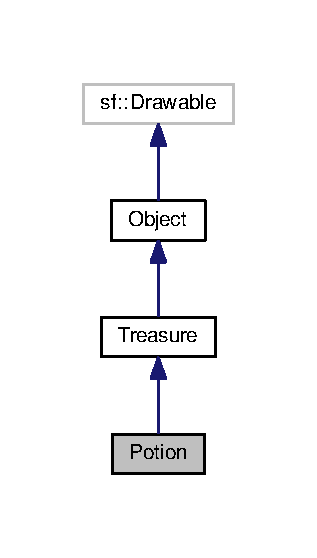
\includegraphics[width=152pt]{classPotion__inherit__graph}
\end{center}
\end{figure}


Collaboration diagram for Potion\+:
\nopagebreak
\begin{figure}[H]
\begin{center}
\leavevmode
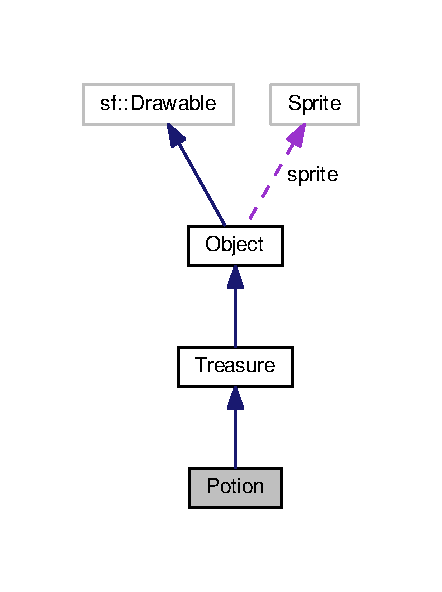
\includegraphics[width=212pt]{classPotion__coll__graph}
\end{center}
\end{figure}
\subsection*{Public Member Functions}
\begin{DoxyCompactItemize}
\item 
\hyperlink{classPotion_a5dbf5d8ebfa702f529feca08359e7105}{Potion} (int x\+\_\+val, int y\+\_\+val, int wid, int val, sf\+::\+Texture \&tex, sf\+::\+Int\+Rect rect)
\item 
virtual void \hyperlink{classPotion_a04d02a0c7c4f5dbeb6062d1399a914c8}{collect} (\hyperlink{classPlayer}{Player} \&player) override
\end{DoxyCompactItemize}
\subsection*{Additional Inherited Members}


\subsection{Constructor \& Destructor Documentation}
\hypertarget{classPotion_a5dbf5d8ebfa702f529feca08359e7105}{\index{Potion@{Potion}!Potion@{Potion}}
\index{Potion@{Potion}!Potion@{Potion}}
\subsubsection[{Potion}]{\setlength{\rightskip}{0pt plus 5cm}Potion\+::\+Potion (
\begin{DoxyParamCaption}
\item[{int}]{x\+\_\+val, }
\item[{int}]{y\+\_\+val, }
\item[{int}]{wid, }
\item[{int}]{val, }
\item[{sf\+::\+Texture \&}]{tex, }
\item[{sf\+::\+Int\+Rect}]{rect}
\end{DoxyParamCaption}
)}}\label{classPotion_a5dbf5d8ebfa702f529feca08359e7105}
A potion the player can collect to restore themselves to full health 
\begin{DoxyParams}{Parameters}
{\em x\+\_\+val} & X coordinate of the potion \\
\hline
{\em y\+\_\+val} & Y coordinate of the potion \\
\hline
{\em wid} & Width of the potion object \\
\hline
{\em val} & Value used to increase the score of the player object \\
\hline
{\em tex} & Tileset texture to create the sprite from \\
\hline
{\em rect} & Area of the tileset to create the sprite from \\
\hline
\end{DoxyParams}


\subsection{Member Function Documentation}
\hypertarget{classPotion_a04d02a0c7c4f5dbeb6062d1399a914c8}{\index{Potion@{Potion}!collect@{collect}}
\index{collect@{collect}!Potion@{Potion}}
\subsubsection[{collect}]{\setlength{\rightskip}{0pt plus 5cm}void Potion\+::collect (
\begin{DoxyParamCaption}
\item[{{\bf Player} \&}]{player}
\end{DoxyParamCaption}
)\hspace{0.3cm}{\ttfamily [override]}, {\ttfamily [virtual]}}}\label{classPotion_a04d02a0c7c4f5dbeb6062d1399a914c8}
Heals the \hyperlink{classPlayer}{Player} object player and sets the \hyperlink{classPotion}{Potion} object's collected variable to true 
\begin{DoxyParams}{Parameters}
{\em player} & The player object that collected the potion \\
\hline
\end{DoxyParams}


Implements \hyperlink{classTreasure_a55f46cc5e888315d78c423e6d0af102d}{Treasure}.



The documentation for this class was generated from the following files\+:\begin{DoxyCompactItemize}
\item 
potion.\+h\item 
potion.\+cpp\end{DoxyCompactItemize}

\hypertarget{classTreasure}{\section{Treasure Class Reference}
\label{classTreasure}\index{Treasure@{Treasure}}
}


Inheritance diagram for Treasure\+:
\nopagebreak
\begin{figure}[H]
\begin{center}
\leavevmode
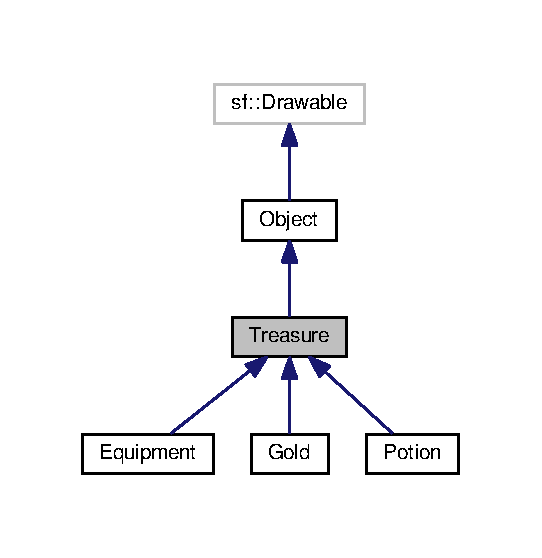
\includegraphics[width=260pt]{classTreasure__inherit__graph}
\end{center}
\end{figure}


Collaboration diagram for Treasure\+:
\nopagebreak
\begin{figure}[H]
\begin{center}
\leavevmode
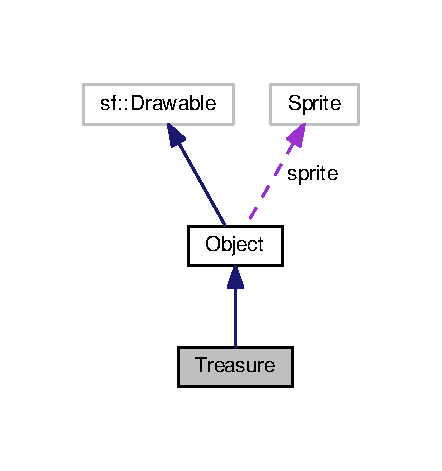
\includegraphics[width=212pt]{classTreasure__coll__graph}
\end{center}
\end{figure}
\subsection*{Public Member Functions}
\begin{DoxyCompactItemize}
\item 
\hyperlink{classTreasure_abdc8e911a0a71955c73847dd726964aa}{Treasure} (int x\+\_\+val, int y\+\_\+val, int wid, int val, sf\+::\+Texture \&tex, sf\+::\+Int\+Rect rect)
\item 
virtual void \hyperlink{classTreasure_a55f46cc5e888315d78c423e6d0af102d}{collect} (\hyperlink{classPlayer}{Player} \&player)=0
\item 
virtual bool \hyperlink{classTreasure_adfa94654619fbe6f193df512e65db083}{active} () const override
\end{DoxyCompactItemize}
\subsection*{Protected Attributes}
\begin{DoxyCompactItemize}
\item 
\hypertarget{classTreasure_a8afb4798dba836b0bf27e06e36932dec}{int {\bfseries value} \{\}}\label{classTreasure_a8afb4798dba836b0bf27e06e36932dec}

\item 
\hypertarget{classTreasure_a08327d05d975fa573f57a1c8887a94dd}{bool {\bfseries collected} \{false\}}\label{classTreasure_a08327d05d975fa573f57a1c8887a94dd}

\end{DoxyCompactItemize}


\subsection{Constructor \& Destructor Documentation}
\hypertarget{classTreasure_abdc8e911a0a71955c73847dd726964aa}{\index{Treasure@{Treasure}!Treasure@{Treasure}}
\index{Treasure@{Treasure}!Treasure@{Treasure}}
\subsubsection[{Treasure}]{\setlength{\rightskip}{0pt plus 5cm}Treasure\+::\+Treasure (
\begin{DoxyParamCaption}
\item[{int}]{x\+\_\+val, }
\item[{int}]{y\+\_\+val, }
\item[{int}]{wid, }
\item[{int}]{val, }
\item[{sf\+::\+Texture \&}]{tex, }
\item[{sf\+::\+Int\+Rect}]{rect}
\end{DoxyParamCaption}
)}}\label{classTreasure_abdc8e911a0a71955c73847dd726964aa}
Abstract class for treasure objects 
\begin{DoxyParams}{Parameters}
{\em x\+\_\+val} & X coordinate of the treasure \\
\hline
{\em y\+\_\+val} & Y coordinate of the treasure \\
\hline
{\em wid} & Width of the treasure object \\
\hline
{\em tex} & Tileset texture to create the sprite from \\
\hline
{\em rect} & Area of the tileset to create the sprite from \\
\hline
\end{DoxyParams}


\subsection{Member Function Documentation}
\hypertarget{classTreasure_adfa94654619fbe6f193df512e65db083}{\index{Treasure@{Treasure}!active@{active}}
\index{active@{active}!Treasure@{Treasure}}
\subsubsection[{active}]{\setlength{\rightskip}{0pt plus 5cm}bool Treasure\+::active (
\begin{DoxyParamCaption}
{}
\end{DoxyParamCaption}
) const\hspace{0.3cm}{\ttfamily [override]}, {\ttfamily [virtual]}}}\label{classTreasure_adfa94654619fbe6f193df512e65db083}
Returns if the object is active or should be deleted, it determines this by looking at the collected variable and returning the opposite of it, since all collected treasures should be removed from the playing field \begin{DoxyReturn}{Returns}
!collected 
\end{DoxyReturn}


Implements \hyperlink{classObject}{Object}.

\hypertarget{classTreasure_a55f46cc5e888315d78c423e6d0af102d}{\index{Treasure@{Treasure}!collect@{collect}}
\index{collect@{collect}!Treasure@{Treasure}}
\subsubsection[{collect}]{\setlength{\rightskip}{0pt plus 5cm}virtual void Treasure\+::collect (
\begin{DoxyParamCaption}
\item[{{\bf Player} \&}]{player}
\end{DoxyParamCaption}
)\hspace{0.3cm}{\ttfamily [pure virtual]}}}\label{classTreasure_a55f46cc5e888315d78c423e6d0af102d}
Function for collecting a treasure object 
\begin{DoxyParams}{Parameters}
{\em player} & The player object that collects the treasure \\
\hline
\end{DoxyParams}


Implemented in \hyperlink{classEquipment_ae420383e1e845e886f60ffa6b6c82312}{Equipment}, \hyperlink{classGold_a15403009146df6691835e27bbd5c0299}{Gold}, and \hyperlink{classPotion_a04d02a0c7c4f5dbeb6062d1399a914c8}{Potion}.



The documentation for this class was generated from the following files\+:\begin{DoxyCompactItemize}
\item 
treasure.\+h\item 
treasure.\+cpp\end{DoxyCompactItemize}

\hypertarget{classWall}{\section{Wall Class Reference}
\label{classWall}\index{Wall@{Wall}}
}


Inheritance diagram for Wall\+:
\nopagebreak
\begin{figure}[H]
\begin{center}
\leavevmode
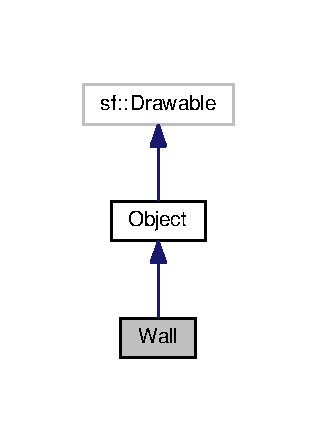
\includegraphics[width=152pt]{classWall__inherit__graph}
\end{center}
\end{figure}


Collaboration diagram for Wall\+:
\nopagebreak
\begin{figure}[H]
\begin{center}
\leavevmode
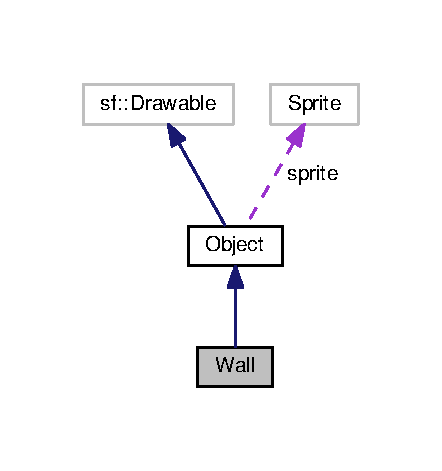
\includegraphics[width=212pt]{classWall__coll__graph}
\end{center}
\end{figure}
\subsection*{Public Member Functions}
\begin{DoxyCompactItemize}
\item 
\hyperlink{classWall_af336438d603b56a880f5dd2d224c4199}{Wall} (int x\+\_\+val, int y\+\_\+val, int wid, sf\+::\+Texture \&tex, sf\+::\+Int\+Rect rect)
\end{DoxyCompactItemize}
\subsection*{Additional Inherited Members}


\subsection{Constructor \& Destructor Documentation}
\hypertarget{classWall_af336438d603b56a880f5dd2d224c4199}{\index{Wall@{Wall}!Wall@{Wall}}
\index{Wall@{Wall}!Wall@{Wall}}
\subsubsection[{Wall}]{\setlength{\rightskip}{0pt plus 5cm}Wall\+::\+Wall (
\begin{DoxyParamCaption}
\item[{int}]{x\+\_\+val, }
\item[{int}]{y\+\_\+val, }
\item[{int}]{wid, }
\item[{sf\+::\+Texture \&}]{tex, }
\item[{sf\+::\+Int\+Rect}]{rect}
\end{DoxyParamCaption}
)}}\label{classWall_af336438d603b56a880f5dd2d224c4199}
Generic wall object on the level 
\begin{DoxyParams}{Parameters}
{\em x\+\_\+val} & X coordinate of the wall \\
\hline
{\em y\+\_\+val} & Y coordinate of the wall \\
\hline
{\em wid} & Width of the wall \\
\hline
{\em tex} & Tileset texture to create the sprite from \\
\hline
{\em rect} & Area of the tileset to create the sprite from \\
\hline
\end{DoxyParams}


The documentation for this class was generated from the following files\+:\begin{DoxyCompactItemize}
\item 
wall.\+h\item 
wall.\+cpp\end{DoxyCompactItemize}

%--- End generated contents ---

% Index
\newpage
\phantomsection
\addcontentsline{toc}{chapter}{Index}
\printindex

\end{document}
